\documentclass{hertieteaching}
\usepackage{bbm}

\title{Content Analysis Dictionaries 2}

\begin{document}

{\setbeamertemplate{footline}{}
\begin{frame}
\maketitle
\end{frame}}
\addtocounter{page}{-1}

% model structure choices
% preprocessing
% strategic considerations

%\begin{frame}{Recap}
%
%
%The \textit{message} of the document is
%$$
%[\theta_1, \ldots, \theta_K]
%$$
%where each element of the message is
%$$
%\theta_k ~=~ P(Z=k) ~=~ \frac{1}{N} \sum^N \mathbbm{1}(Z_i = k)
%$$
%
%Quite generally, the optimal \textit{estimator} for this is 
%\begin{align*}
%\hat{\theta}_k & ~=~ \frac{1}{N}\sum^N_i P(Z_i=k \mid \{ W \}) \\
%              & ~=~ \frac{1}{N}\sum^N_i P(Z_i=k \mid W_v[i]) & \text{(because we use a content analysis dictionary)}
%\end{align*}
%where we've replaced the unknown $Z_k$ with our best guess given the word type.
%
%
%\end{frame}
%\begin{frame}{Recap}
%Why is this the optimal estimator?
%
%Example (simple):
%\begin{itemize}
%  \item If topic $k$ is the \textit{only} one that generate words of type $W_{v[i]}$, that is if
%  $$
%  P(W_{v[i]} \mid Z = k) = 1
%  $$
%  then definitely $P(Z_k = k \mid W_{v[i]}) = 1$
%  \item So we should count 1 for topic $k$ 
%\end{itemize}
%
%\end{frame}
%\begin{frame}{Recap}
%
%Example (trickier): 
%\begin{itemize}
%  \item Topics $j$ and $k$ generates $W_{v[i]}$, e.g. 
%  \begin{align*}
%    P(W_{v[i]} \mid Z = k) &= 0.03 & 
%    P(W_{v[i]} \mid Z = j) &= 0.01
%  \end{align*}
%  but \textit{no other topics} do. 
%\end{itemize}
%then Rev. Bayes says
%\begin{align*}
%  P(Z=k \mid W_{v[i]}) & ~=~ P(W_{v[i]} \mid Z = k) P(Z=k) / P(W_{v[i]})\\
%\intertext{and if we don't have a reason before seeing any words  to think topic $k$ is more or less frequent than $j$}
%  & ~=~ \frac{0.03}{(0.03 + 0.01)} ~=~ 3/4
%\end{align*}
%Since only two topics generate this word the other topic gets the remaining $1/4$
%\end{frame}
%
%\begin{frame}{Recap}
%
%In short:
%\begin{itemize}
%  \item We \textit{redistributed} one count across the two topics that might of generated it, in proportion to how likely they were to have generated it.
%\end{itemize}
%We cannot do better than this! \pause We can do worse though.
%
%Best case scenario:
%\begin{itemize}
%  \item Our dictionary sees this word and assigns it to topic $k$ (because that's most likely) then our measurement error is\ldots 1/4
%\end{itemize}
%
%
%
%  
%  
%\end{frame}


%\begin{frame}{Recap}

%\begin{frame}{}
%  
%  with probability 0.1, topic $j$ generates it with probability 0.025, and no other topics generate it at all, then
%  \begin{align*}
%  P(W_{v[i]} \mid Z = k) = 3/4 & ~~\text{and}~~ P(W_{v[i]} \mid Z = j) = 1/4
%  \end{align*}
%\end{itemize}
%
%\end{frame}
%
%if there's a 50\% chance that any a $W_i$ was generated by the $k$-th topic, then we count it 50%
%
%
%\frac{1}{N}\sum^N_i \textbb{I}[Z_i=k]
%
%
%
%
%First count up all the `hits', where $Z=k$
%$$
%Z_k ~=~ \sum^N_{i} P(Z = k \mid W_i)
%$$
%then divide by the sum
%$$
%\hat{\theta}_k ~=~ \frac{Z_k}{\sum^K_{j} Z_j}
%$$
%and that's our estimate of the document content
%
%
%
%
%A simple example, elaborating on the measurement error we saw in the previous lecture
%
%Let's work with a tiny subset of the \textcite{Laver.Garry2000} dictionary. This time we'll use some words from the `neutral' category too
%
%\medskip
%\begin{center}
%\begin{tabular}{ll} \toprule
%  \textbf{state reg}     & \textbf{centrist} & \textbf{market econ} \\ \midrule
%          accommodation  & accountants & assets\\
%          age            & bargaining  & bid\\
%          ambulance      & electricity & choice*\\
%          \ldots         & \ldots 
%\end{tabular}
%\end{center}
%
%\end{frame}
%
%\begin{frame}{Recap}
%
%Target 
%
%
%\end{frame}
%
%\begin{frame}{Topics}
%
%\begin{center}
%\begin{tikzpicture}
%\node(W) at (1.5,0)  [var,label=below:$W$]{};
%\node(Z) at (3,0)  [lat,label=below:$Z$]{};
%\draw(Z) -- (W);
%\draw[gray](1,-0.75) rectangle (3.75,0.5){};
%\node[gray] at (4,-0.6){\small N};
%\node(theta) at (4,1)  [lat,label=right:$\theta$]{};
%\draw(theta) -- (Z);
%\node(beta) at (-0.25, 0) [var,label=below:$B$]{};
%\draw(beta) -- (W);
%\draw(-0.75,-0.75) rectangle (0.5,0.5)[gray];
%\node(labk) at (-0.95,-0.6)  []{{\color{gray}\small K}};
%
%\end{tikzpicture}
%\end{center}
%
%
%$B$ is a `dictionary' that explains how often each word should be generated in each of the $K$ topics
%\begin{itemize}
%  \item An entry in the dictionary $B$ is a vector of word generation probabilities $\beta_k$ 
%\end{itemize}
%This week we will assume we \textit{know} $B$
%
%\pause
%Strictly speaking we will assume that we know enough about its \textit{inverse} $W \longrightarrow Z$ to say
%\begin{itemize}
%  \item for each word $W$, what its $Z$ is.
%\end{itemize}
%
%\end{frame}

\nocite{Mikhaylov.etal2011}

\begin{frame}{Solutions: Some theological approaches}

\pause

\centerline{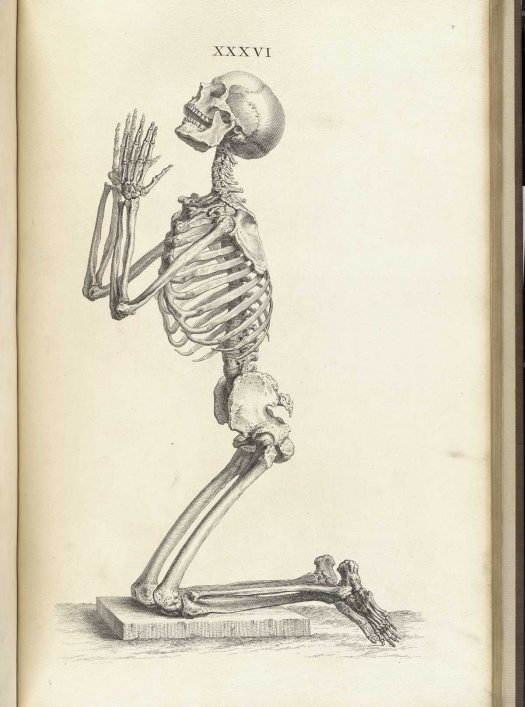
\includegraphics[scale=0.3]{pictures/praying-skeleton}}

\centerline{``Thoughts and prayers''}

\end{frame}

\begin{frame}{How bad is it?}

\begin{itemize}
  \item \textit{Recall}: the proportion of words used that way that are in your dictionary
  \item \textit{Precision}: the proportion of words used the way your dictionary
  assumes they are used
\end{itemize}

\end{frame}

\begin{frame}{Precision and recall}

\textit{Every} field reinvents this distinction:

\begin{itemize}
\item
  precision and recall
  \item
  specificity and sensitivity
  \item
  users and producer's accuracy
  \item
  type 1 and type 2 error
  \item sins of omission and sins of commission
\end{itemize}

\end{frame}

\begin{frame}{Precision}

Keyword in context analyses (KWIC) allow you to scan all contexts of a word 

\begin{itemize}
\item
  How many of them \textit{are} the sense or usage you want?
\end{itemize}

Let's take a look at \texttt{benefit*} as a `pro government intervention in the economy' word

\end{frame}

\begin{frame}{}

\footnotesize
\begin{table}[ht]
\centering
\begin{tabular}{rlll}
  \hline
 & pre & keyword & post \\ 
  \hline
1 & also keep all the other & benefits & that pensioners currently receive , \\ 
  2 & regulation will have to have & benefits & exceeding costs , and regulations \\ 
  3 & and Controlled Immigration Britain has & benefited & from immigration . We all \\ 
  4 & positive contribution But if those & benefits & are to continue to flow \\ 
  5 & Northern Ireland brings & benefits & to all parts of our \\ 
  6 & their home , will also & benefit & first-time buyers . Empowering individuals \\ 
  7 & you help yourself ; you & benefit & and the country benefits . \\ 
  8 & you benefit and the country & benefits & . So now , I \\ 
  9 & result of our tax and & benefit & measures compared to 1997 . \\ 
  10 & result of personal tax and & benefit & measures introduced since 1997 , \\ 
  11 & , the savings on unemployment & benefits & will go towards investing more \\ 
  12 & trebled the number on incapacity & benefits & . We will help 17 \\ 
  13 & Work programme and reform Incapacity & Benefit & , with the main elements \\ 
  14 & main elements of the new & benefit & regime in place from 2008 \\ 
  15 & stronger penalties . To the & benefit & of business and household consumers \\ 
  16 & effective directive to provide real & benefits & to consumers and new opportunities \\ 
  17 & better.We are examining the potential & benefits & of a parallel Expressway on \\ 
  18 & ways to lock in the & benefit & of new capacity . We \\ 
  19 & are determined to spread the & benefits & of enterprise to every community \\ 
  20 & to get ahead , to & benefit & from improving public services\\
   \hline
\end{tabular}
\end{table}
\normalsize

\end{frame}

\begin{frame}{Precision}

Of the 20 instances, these are (arguably)
\begin{itemize}
  \item 6 used the way we expect from the topic
  \item 3 used in the opposite sense: anti-government intervention in the economy
  \item 11 used in ways that are neither
\end{itemize}

So\ldots 0.3 correct, 0.15 mistaken, and 0.55 unrelated `noise'
\begin{itemize}
  \item Perhaps not an amazing choice
\end{itemize}

There are two kinds of precision failures here with different consequences
\begin{itemize}
  \item Mistaking an \textit{topic-unrelated} word for this topic (11 of these)
  \item Mistaking a word used in the sense of a \textit{different} topic for this one (3 of these)
\end{itemize}

The first mistake does not really harm precision, but the second does

\end{frame}

\begin{frame}{Recall}

Bad recall is a mixture of two problems
\begin{itemize}
  \item Assigning words to a topic that are mostly used for a different one: $P(W \mid Z=k)<P(W \mid Z=j)$ but we assigned it to $k$ anyway
  \item Failing to assign a topic-informative word to any topic: Dictionary says $P(W \mid Z=k)=0$, but it's not. This is about \textit{coverage}
\end{itemize}

Let's consider coverage first

\end{frame}
\begin{frame}{Coverage}

One possible checking procedure:
\begin{itemize}
  \item Take a random matched sample of words not in the dictionary but present in the corpus e.g. match each dictionary word to another of the same frequency
  \item Examine their KWICs to see if they should have been assigned to a topic
\end{itemize}
If we were feeling even more energetic
\begin{itemize}
  \item Assign them their most likely topic manually
  \item Compare this $\tilde{\theta}$ to the dictionary's own estimate $\theta$
  \item These should not be wildly different
\end{itemize}
  
\end{frame}

\begin{frame}{Recall}

The other kind of mistake is difficult because the natural procedure is
\begin{itemize}
  \item Assign \textit{every word} (or at least every instance of a word that the dictionary knows about in a document) to a topic
  \item For each topic, see what proportion of times  the dictionary agrees it is in that topic
\end{itemize}
This also promises to be very tiring.

\end{frame}


\begin{frame}{Using precision to estimate recall}


However, two facts may help us:
\begin{itemize}
  \item We have a tireless computer available
  \item Recall and precision relate $P(W \mid Z)$ and $P(Z \mid W)$ respectively
  \item \ldots and we know how
\end{itemize}

Let's call the \textit{true} topic of a word $Z$ as before, and the \textit{dictionary's idea of the topic} of a word $\hat{Z}$ because it's kind of an estimate of that. So,
\begin{align*}
\text{Recall:} & ~~~~ \sum^K_k P(\hat{Z}=k \mid Z=k)\\
\text{Precision:} & ~~~~ \sum^K_k P(Z=k \mid \hat{Z}=k)
\end{align*}

\end{frame}

\begin{frame}{Using precision to estimate recall}

If we have a sense of dictionary topic precision, could we use it to get a sense of dictionary topic recall? \pause Why yes, by borrowing methods from \textcite{King.Lowe2003}.
\pause

According to the Rev. Bayes
\begin{align*}
P(\hat{Z}=k \mid Z=k) &~=~ \frac{P(Z=k \mid \hat{Z}=k) P(\hat{Z}=k)}{\sum^K_j P(Z=j \mid \hat{Z}=j) P(\hat{Z}=j)} \\
                      &~=~ P(Z=k \mid \hat{Z}=k) \frac{P(\hat{Z}=k)}{P(Z=k)}& \text{(recall is reweighted precision)}\\
                      &~\propto~ P(Z=k \mid \hat{Z}=k) P(\hat{Z}=k) 
\end{align*}
Conveniently
\begin{itemize}
  \item we don't need the denominator because it only ensure the recall measures add to one
  \item We can get $P(\hat{Z}=k)$ by running the dictionary over the entire corpus
\end{itemize}
  
\end{frame}

\begin{frame}{Perspective}

Precision and recall are useful, but we are most interested in the \textit{consequences} of being wrong

Previously: consequences for a left-right ideology measure from \textcite{Laver.Garry2000}


\bigskip

Let's look at a related conflict-cooperation score assigned by experts to dictionary `topics' \parencite{King.Lowe2003}

A machine coding system `read' Agence France Press leads on the Bosnian wars and generated event data
\begin{itemize}
  \item Who did what to whom when
\end{itemize}
We were interested in evaluating the `what'

\begin{itemize}
  \item Topics are event types in a large ontology of international events
  \item topic \textit{scores} represent how conflictual or cooperative that event is
  \item Some topic categorization mistakes will matter more than others
\end{itemize}

	
\end{frame}
\begin{frame}{Event topics}

\centerline{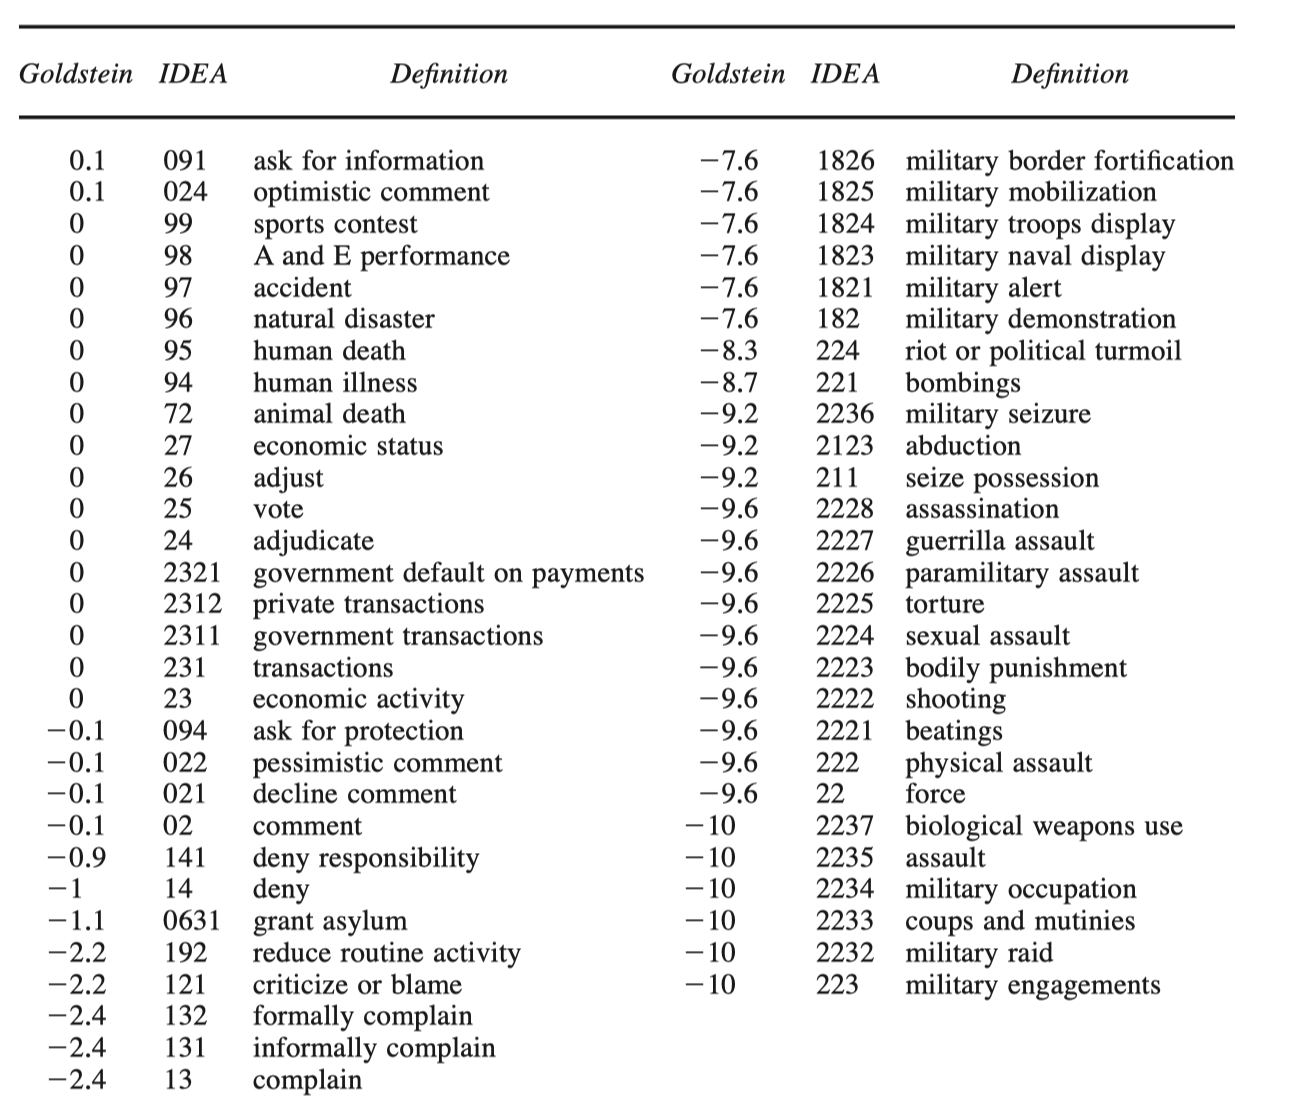
\includegraphics[scale=0.4]{pictures/kinglowe2}}
\end{frame}

\begin{frame}{Topic scores}

\centerline{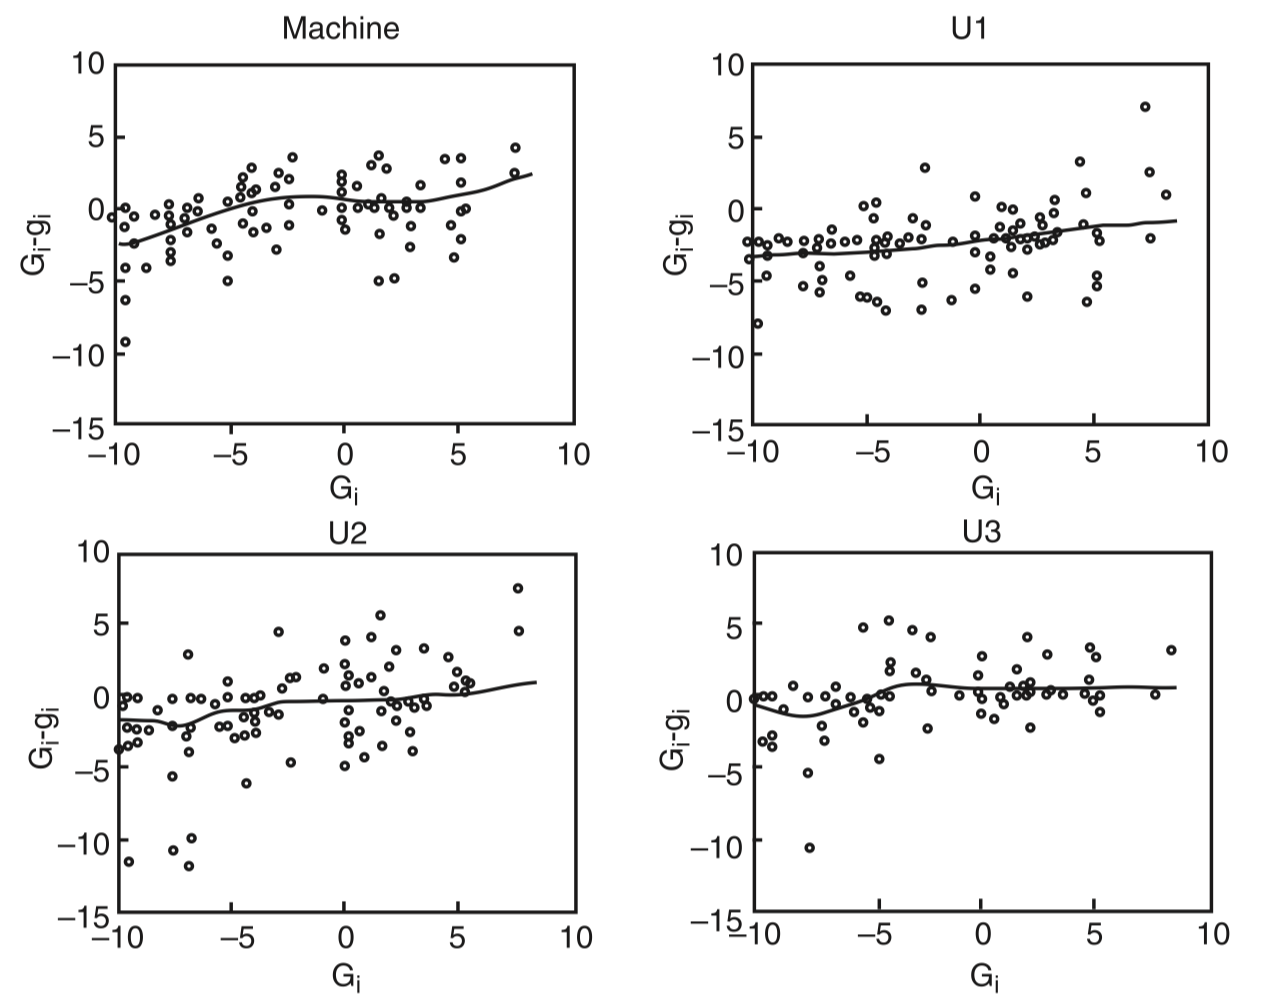
\includegraphics[scale=0.4]{pictures/kinglowe}}
\end{frame}

\begin{frame}{Topic scores}

Not bad (or at least not bad relative to undergraduate coders)

All the evaluation principles we've seen here apply to 
\begin{itemize}
  \item document classifiers
  \item content analysis dictionaries
  \item human coders
\end{itemize}
Nothing is more practical than a good theory\ldots 

\pause
\bigskip


Next week we'll see how we learn dictionaries rather than write them
\begin{itemize}
  \item but all the same considerations will apply
\end{itemize}


\end{frame}



%%%%%%%

%\begin{frame}{Working from a dictionary}
%
%Under reasonable assumptions
%\begin{itemize}
%\item
%  A observed category proportions are generated by a \emph{mixture} of
%  categories
%\item
%  The weights for this mixture are the true category proportions
%  \(P(Z=k) = \theta\)
%\end{itemize}
%
%\[
%P(W) = \sum^K_k {P(W \mid Z=k)} P(Z=k)
%\]
%
%\end{frame}
%
%\begin{frame}{Correction}
%
%
%But back to words and their categories\ldots{}
%
%\[
%P(W) = \sum^K_k {P(W \mid Z=k)} P(Z=k)
%\]
%
%If we knew about the error process \(P(W \mid Z=k)\), we could
%\emph{back out} the true proportions
%
%\end{frame}
%
%\begin{frame}{Alternative approach}
%
%\begin{center}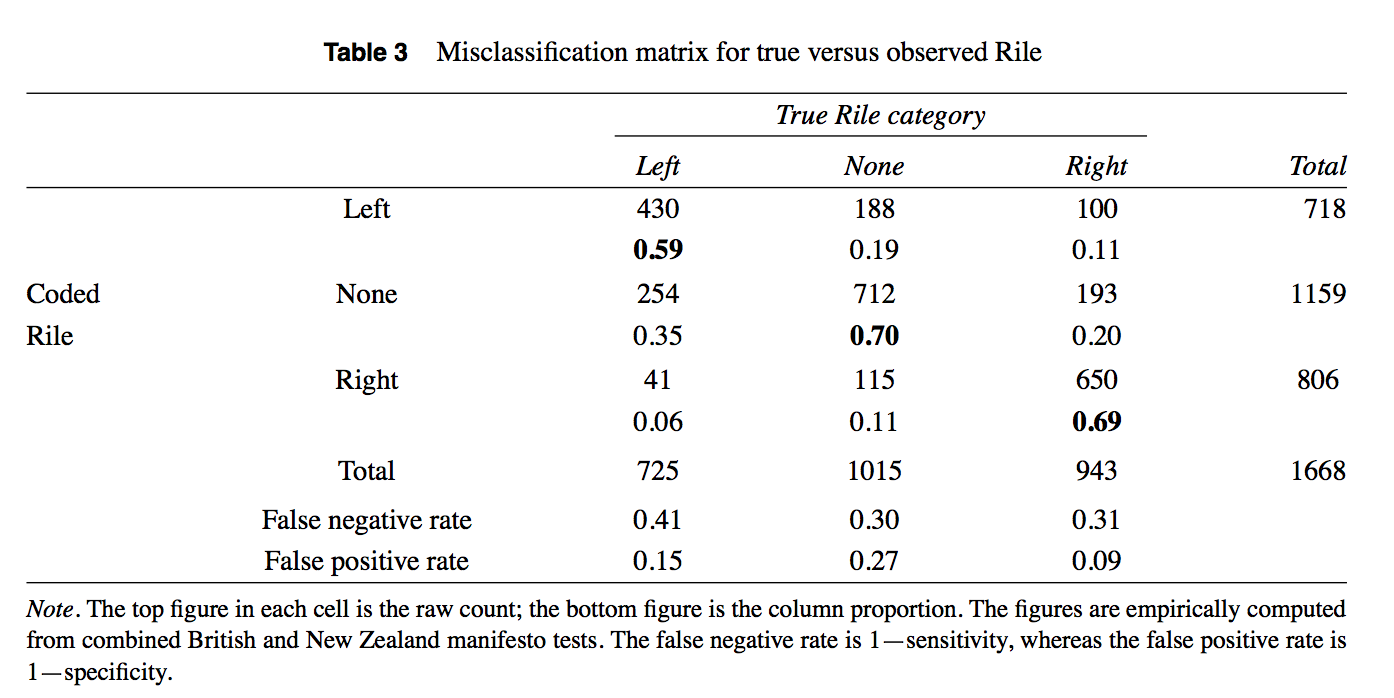
\includegraphics[width=0.8\linewidth]{pictures/slava-rile3} \end{center}
%
%From \textcite{Mikhaylov.etal2011}
%
%\end{frame}
%
%\begin{frame}{A general purpose linear approach}
%\protect\hypertarget{a-general-purpose-linear-approach}{}
%
%The category proportions are \[
%P(W) = \sum^K_k {P(W \mid Z=k)} P(Z=k)
%\] has the form \[
%P = E \theta
%\] where \(P\) are the coded proportions and \(E\) is the \(V \times K\)
%coder error matrix, so \[
%\theta = \text{E}^{-1} P
%\] Typically we don't exactly know \text{E} so the result is an
%approximation
%
%\end{frame}
%
%\begin{frame}{An application to human sentence coders}
%\protect\hypertarget{an-application-to-human-sentence-coders}{}
%
%Application to Mikhaylov et al.'s subjects coding New Zealand party
%manifestos.
%
%\begin{longtable}[]{@{}lllll@{}}
%\toprule
%& true & L & N & R\tabularnewline
%\midrule
%\endhead
%code & L & 430 & 188 & 100\tabularnewline
%& N & 254 & 712 & 193\tabularnewline
%& R & 41 & 115 & 650\tabularnewline
%\bottomrule
%\end{longtable}
%
%\end{frame}
%
%\begin{frame}{Convert to error probabilities}
%\protect\hypertarget{convert-to-error-probabilities}{}
%
%Errors: \(E\)
%
%\begin{table}[ht]
%\centering
%\begin{tabular}{rrrr}
%  \toprule
% & L & N & R \\ 
%  \midrule
%L & 0.59 & 0.19 & 0.11 \\ 
%  N & 0.35 & 0.70 & 0.20 \\ 
%  R & 0.06 & 0.11 & 0.69 \\ 
%   \bottomrule
%\end{tabular}
%\end{table}
%
%\pause
%
%Inverted: \(E^{-1}\)
%
%\begin{table}[ht]
%\centering
%\begin{tabular}{rrrr}
%  \toprule
% & L & N & R \\ 
%  \midrule
%L & 2.00 & -0.50 & -0.16 \\ 
%  N & -1.00 & 1.75 & -0.37 \\ 
%  R & 0.00 & -0.25 & 1.52 \\ 
%   \bottomrule
%\end{tabular}
%\end{table}
%
%\pause
%
%\(\theta\) = 0.27, 0.38, 0.35
%
%\pause
%
%Observed P = 0.27, 0.43, 0.3
%
%\end{frame}
%
%\begin{frame}{Implications for derived measurements}
%\protect\hypertarget{implications-for-derived-measurements}{}
%
%If {[}L, N, R{]} were {[}20, 0, 10{]}
%
%\begin{itemize}
%\tightlist
%\item
%  true position: -0.33 on our previous left-right scale, ignoring N
%\end{itemize}
%
%Under measurement error we would \emph{expect} to see about {[}13, 9,
%8{]}
%
%\begin{itemize}
%\tightlist
%\item
%  an attenuated -0.24 on our previous scale
%\end{itemize}
%
%Correcting this with the correct error matrix would recover the right
%proportions, and so the right position
%
%\end{frame}
%
%\begin{frame}{Implementations and limitations}
%\protect\hypertarget{implementations-and-limitations}{}
%
%Hopkins and King (2010) and King and Lu (2008) implement this strategy
%
%\pause
%
%When coder errors are only \emph{estimated} the result hold in
%expectation.
%
%The tradeoff is between
%
%\begin{itemize}
%\tightlist
%\item
%  errors coders make
%\item
%  errors we make estimating the errors coders make\ldots{}
%\end{itemize}
%
%\end{frame}
%
%\begin{frame}{Implementations and limitations}
%\protect\hypertarget{implementations-and-limitations-1}{}
%
%Linearity means we sometimes estimate proportions outside {[}0,1{]}
%
%Alternatively we can assign distributions and work with the original
%structure \[
%{P(W)} = \sum^K_k {P(W \mid Z=k)} P(Z=k)
%\] and that is exactly what topic models do.
%
%\end{frame}

%%%%%%%

\begin{frame}[allowframebreaks]
\frametitle{References}
\printbibliography	
\end{frame}


\end{document}
